% Created with jtex v.1.0.20
%%%%%%%%%%%%%%%%%%%%%%%%%%%%%%%%%%%%%%%%%%%%%%%%%%%%%%%%%%%%
%%% LaPreprint: PREPRINT TEMPLATE
%%%%%%%%%%%%%%%%%%%%%%%%%%%%%%%%%%%%%%%%%%%%%%%%%%%%%%%%%%%%

% Here I could talk about what one should do in this document.
% Instead I'll refer you to the explore on your own and check the Github Repo. :-)
% Line spacing is 1.2 by default (can't be smaller).

%%%%%%%%%%%%%%%%%%%%%%%%%%%%%%%%%%%%%%%%%%%%%%%%%%%%%%%%%%%%
%%% PREAMBLE
%%%%%%%%%%%%%%%%%%%%%%%%%%%%%%%%%%%%%%%%%%%%%%%%%%%%%%%%%%%%

% Declare document class
\documentclass[9pt,Preprint]{lapreprint}
% Choose between "biorxiv", "medrxiv", "arxiv" and "chemrxiv". Otherwise defaults "Preprint".
% Choose between "blue" and "red" colour scheme. Defaults to "blue".
% Use the "onehalfspacing" option for 1.5 line spacing.
% Use the "doublespacing" option for 2.0 line spacing.
% Use the "lineno" option for line numbers.
% Use the "endfloat" option to place floats after the bibliography.
% Use the "secnum" option to have include numbers.

% Import packages
% \usepackage{lipsum}     % Required to insert dummy text
\usepackage[version=4]{mhchem} % For chemical notation
\usepackage{siunitx}    % For SI units
\usepackage{pdflscape}  % For putting pages in landscape mode
\usepackage{rotating}   % For rotating specific elements
\usepackage{textgreek}  % Greek symbols
\usepackage{gensymb}    % Symbols
\usepackage[misc]{ifsym} % For the \Letter symbol
\usepackage{orcidlink}  % For the \orcidlink
\usepackage{listings}   % For inserting code chunks
\usepackage{colortbl}   % For Knitr table colouring
\usepackage{tabularx}   % For making Knitr tables compatible
\usepackage{longtable}  % For multi-page tables
\usepackage{subcaption}
\usepackage{multirow}
\usepackage{snotez}     % For sidenote environments. enotez for endnotes
\usepackage{csquotes}   % For language-based quote rules (helps BiBLaTeX)



% Make declarations
\DeclareSIUnit\Molar{M}

% Please note that these options may affect formatting.

%%%%%%%%%%%%%%%%%%%%%%%%%%%%%%%%%%%%%%%%%%%%%%%%%%%%%%%%%%%%
%%% BIBLIOGRAPHY
%%%%%%%%%%%%%%%%%%%%%%%%%%%%%%%%%%%%%%%%%%%%%%%%%%%%%%%%%%%%
\usepackage[			% use biblatex for bibliography
	backend=biber,      % use biber or bibtex backend
    style=authoryear,   % choose style
	natbib=true,		% allow natbib commands
	hyperref=true,	    % activate hyperref support
	alldates=year,      % only show year (not month)
]{biblatex}

% Just avoiding some rogue fields that cause issues with certain styles
\AtEveryBibitem{
    \clearfield{urlyear}
    \clearfield{urlmonth}
    \clearlist{language}
}

% Update to your bibliography file
\addbibresource{main.bib}


%%%%%%%%%%%%%%%%%%%%%%%%%%%%%%%%%%%%%%%%%%%%%%%%%%%%%%%%%%%%
%%% ARTICLE SETUP
%%%%%%%%%%%%%%%%%%%%%%%%%%%%%%%%%%%%%%%%%%%%%%%%%%%%%%%%%%%%

% Paper title
\title{CT scan reconstruction using machine learning}

% Authors - you can use \orcidlink{} and \authfn{} - see contribution note
\author[]{Luuk Froling}

% Affiliations

% Other metadata. Feel free to add your own
\metadata[]{Keywords}{Finite volume; Direct current; Resistivity; DC equations}


% Surname of the lead author(s) for the running footer
\leadauthor{Luuk Froling}
\shorttitle{Written by Luuk Fröling}

%%%%%%%%%%%%%%%%%%%%%%%%%%%%%%%%%%%%%%%%%%%%%%%%%%%%%%%%%%%%
%%% ARTICLE START
%%%%%%%%%%%%%%%%%%%%%%%%%%%%%%%%%%%%%%%%%%%%%%%%%%%%%%%%%%%%

\begin{document}
\maketitle


\textbf{Author:} Luuk Fröling

\subsection{abstract}

This will be the abstract

\subsection{Introduction}

This will be the introduction

\begin{itemize}
\item important to focus this research is about \textbf{speedup} not about accuracy
\end{itemize}

\subsection{Theory}

\subsubsection{Basics CT scans}

A computed tomography (CT) scanner is an imaging device that uses x-rays to create cross-sectional images of an object. It consists of an x-ray source and a detector placed at a distance from eachother. During scanning, both the source and the detector will rotate around the object to be imaged in steps. For each step, the source emits x-rays that pass through the object; the transmitted photons are measured by the detector. The number of detected photons at position i along the detector is given by:

\begin{equation}
\label{first }
\hat{y}_i  = N_0 \cdot \exp\left(-\int \mu(x, E) \, dx\right)
\end{equation}

where $N_0$ is the number of the x-rays entering emitted by the source, $\mu(x, E)$ is the linear attenuation coefficient and the integral in the exponent represents the cumulative attenuation along the x-ray path. $\mu(x, E)$ describes how many of the incoming x-rays are absorbed per unit of length, which depends on both the material of the object and the energy of the x-ray \parencite{kamalian2016ct_principles}.

By rotating the source and detector around the object and recording measurements at multiple angles, a sinogram can be created. A sinogram is a 2D plot where each row corresponds to a detector reading at a specific projection angle.

\begin{figure}[!htbp]
\centering
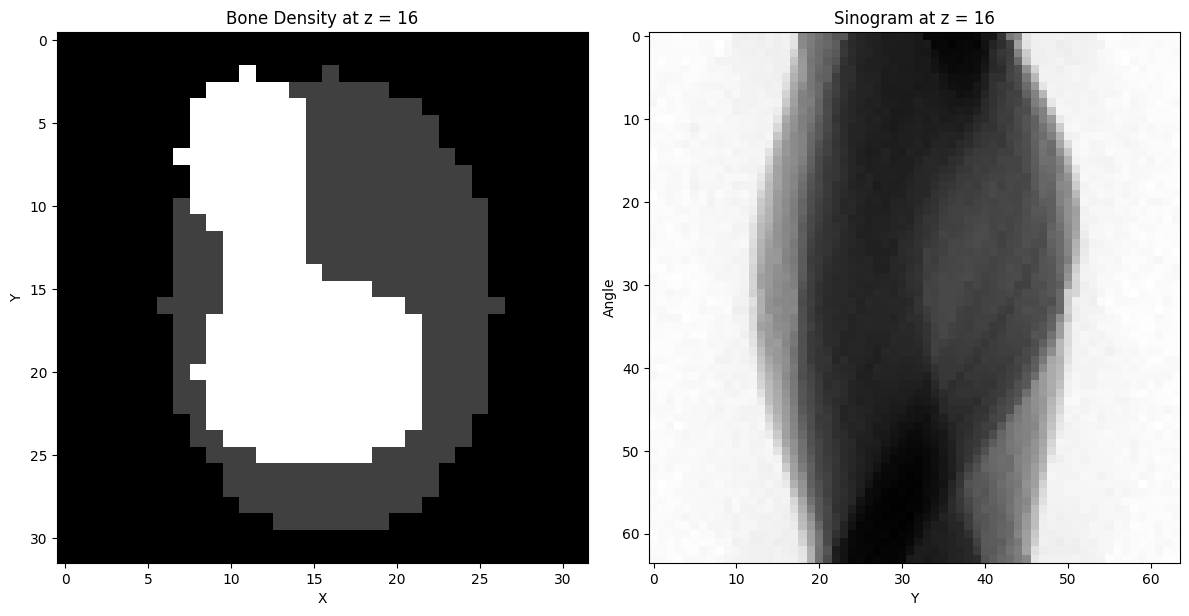
\includegraphics[width=0.7\linewidth]{files/b976b4c5294674aa189b37fdcfeb40f7.png}
\caption[]{\textit{left:} a 32x32 pixel phantom representing varying bone densities. \textit{right} corresponding sinogram with 64 projection angles. The lighter regions in the sinogram indicate higher photon counts. The CT energy used was [TODO].}
\label{phantomSinogram}
\end{figure}

A phantom and a corresponding sinogram can be seen in Figure~\ref{phantomSinogram}. The phantom is a 32x32 image, where each pixel represents a part of the phantom with a specific bone density. Lighter coloured areas having a higher bone density where darker areas have a lower bone density. On the right is the corresponding sinogram which consists of 64 measurements of $\hat{y}_i$ at different angles. The lighter parts of the sinogram correspond to more detected photons.

\subsubsection{Cone beam CT scan}

The sinogram in Figure~\ref{phantomSinogram} is true for a 1D detector, where we construct a single slice. A cone beam CT scan uses a source emitting x-rays in a cone-beam shape, which can be detected on a 2D flat-panel detector \parencite{venkatesh2017cbct}.

\begin{figure}[!htbp]
\centering
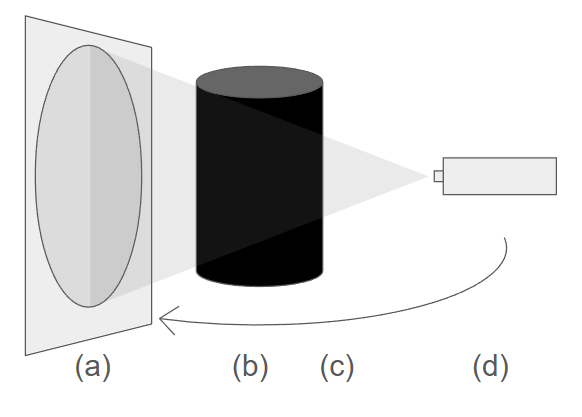
\includegraphics[width=0.5\linewidth]{files/cone_beam_ct-cf60e2b0345375bb14b01c570192d07f.png}
\caption[]{A schematic drawing of a cone-beam CT scan: (a) the 2D detector panel, (b) the phantom, (c) rotation direction of the source-detector pair (d) the x-ray source.}
\label{cone_beam}
\end{figure}

Figure~\ref{cone_beam} shows a cone beam CT scan setup, where both the detector and the source rotate around the object to acquire a set of 2D projection images at multiple angles. these measurements are known as rays.

The relationship between the object and the measured rays can be described by a projection matrix $A$. This matrix has dimensions $M \times N$ where $N$ is the number of voxels in the object and $M$ is the number of rays (measurements) collected by the detector. Each element $a_{mn}$ of the matrix is the contribution of the nth voxel of the object to be imaged to the mth ray of the detector \parencite{Yang2017ProjectionMatrix}. The measured projections can thus be modeled as:

\begin{equation}
y = Ax
\end{equation}

where $x$ is the vectorised representation of the voxel values and $y$ contains the corresponding ray measurements. This formulation is will be used by the reconstruction algorithms during the simulations.

\subsubsection{Detector types}

Current CT scanners use an energy integrating detector (EID) \parencite{marth2023photon}. An EID measures the intensity of the incoming x-rays by a two-step process: scintillation followed by photodetection. The scintillator will absorb the x-rays which have passed through the body and emit light in the visible spectrum. These re-emitted photons can be detected by photodetectors located underneath the scintillator. Due to the difference in energy of the incoming x-ray and the emitted visible light, multiple photons can be re-emitted. To measure a signal, EIDs integrate over time which loses all energy dependent information \parencite{taguchi2013photon}.

\begin{figure}[!htbp]
\centering
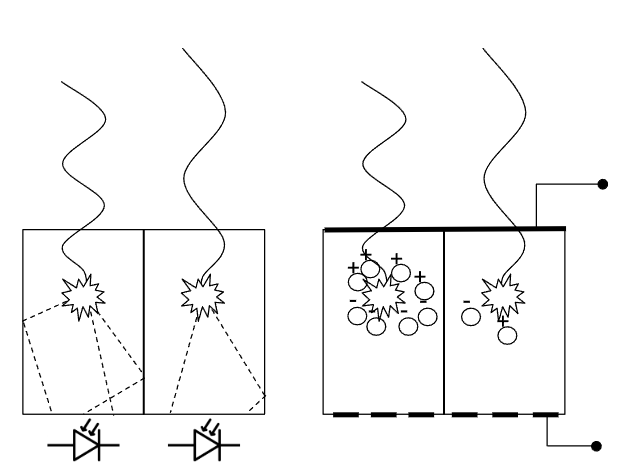
\includegraphics[width=0.5\linewidth]{files/detectorTypes-8bd48a755bc03e91c0cd2be80c4a4001.png}
\caption[]{\textit{left:} An EID where the incoming x-rays are absorbed within the scintillator. Several photons within the visible light spectrum are re-emitted which can be measured by the photodiodes located below the scintillator. \textit{right:} A PCD where incoming x-rays create electron-hole pairs in a semiconductor. This creates a current between the top and bottom of the semiconductor which can be measured by electrodes, preserving energy dependent information.}
\label{detectors}
\end{figure}

Photon-counting detector (PCD) CT scans improve the measurements by directly transforming the incoming CT scans into an energy-dependent signal which can be measured as illustrated in Figure~\ref{detectors}. The incoming x-rays will be absorbed in a semiconductor layer, forming electron-hole pairs which generate an electric signal proportional to the energy of the absorbed photon. Unlike EIDs, this allows the detector to retain energy-dependent information for each photon.

\begin{figure}[!htbp]
\centering
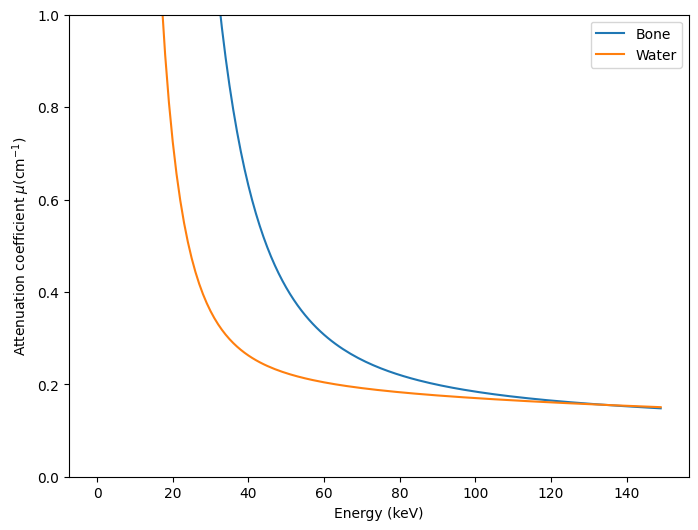
\includegraphics[width=0.7\linewidth]{files/64ccdbd7840b97b269bc4a429597ebd6.png}
\caption[]{The linear attenuation coefficient ($\mu$) of bone (blue) and water (orange) plotted as a function of the incoming x-ray photon energy. The different energy-dependent attenuation behaviour enables material differentiation in photon-counting CT.}
\label{matatt}
\end{figure}

The linear attenuation coefficient used in equation (\ref{first}) depends on the material and the x-ray energy used as illustrated by the attenuation curves in Figure~\ref{matatt}. Using a source emitting x-rays at a range of energies, energy bins can be generated by the PCD where each bin contains energy-specific measurements \parencite{pcd2022}. This enables the differentiation between materials with similar densities which would otherwise appear similar in conventional CT scans using EIDs.

\subsubsection{Material decomposition}

Since different materials attenuate x-rays differently across the energy spectrum, PCD-CT can be used to distinguish between different tissue types within the body. To simulate this process and to describe the attenuation properties of different materials in a phantom, material decomposition is used \parencite{mechlem2018joint}. In this work, material decomposition models each material in the phantom as a linear combination of two basis materials: bone and water.

The reconstructed image of a PCD CT scan will therefore consist of 2 images, one displaying the bone density and one displaying water density. The linear attenuation coëfficient of any material within the phantom can then be described as:

\begin{equation}
\label{muE}
\mu(E) = \sum_{b=1}^{B} A_b f_b(E)
\end{equation}
where $A_b$ is the line integral of material b and $f^b(E)$ describes the attenuation coefficient of the basis material b. Combining equation (\ref{first}) and (\ref{muE}) gives an expression for the photon count at the detector:

\begin{equation}
\hat{y}_i = \int_0^{\infty} \phi_{\text{eff},i}(E) \exp\left( - \sum_{b=1}^{B} A_b^i f_b(E) \right) \, dE
\end{equation}

where $\phi_{\text{eff},i}(E)$ is an effictive x-ray spectrum which includes all source and detector effects.

\subsubsection{Projection algorithms [Work in progress]}

\begin{itemize}
\item brief overview backprojection  \parencite{zeng2001image}


\item list issues


\item brief overview itterative approach (with references to Mechlem)


\item positives


\item negatives
\end{itemize}

part of abstract: ``g. They require a specific
reconstruction process, consisting of two steps: material decomposition and tomographic
reconstruction. Image-based methods perform reconstruction, then decomposition, while
projection-based methods perform decomposition first, and then reconstruction. As an alternative,
`one-step inversion' methods have been proposed, which perform decomposition and reconstruction
simultaneously. Unfortunately, one-step methods are typically slower than their two-step
counterparts, and in most CT applications, reconstruction time is critical. This paper therefore
proposes to compare the convergence speeds of five one-step algorithms.'' \parencite{mory2018comparison}

itterative unet \parencite{ge2023mb}

\subsubsection{Machine learning - Neural networks}

Neural networks are a subset of machine learning and play a crucial role in deep learning algorithms. Every neural network consists of nodes stacked in layers: an input layer, one or more hidden layers and an output layer.

\begin{figure}[!htbp]
\centering
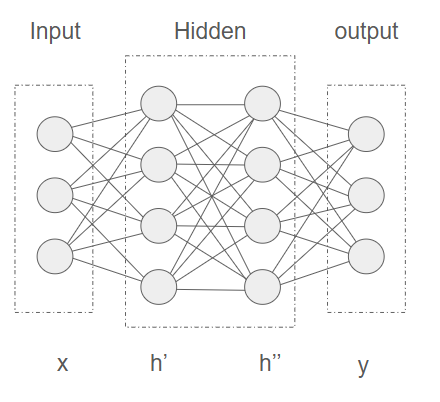
\includegraphics[width=0.7\linewidth]{files/neuralnetwork-4eb553254a7d8035ac96a98b9131098f.png}
\caption[]{A neural network consisting of 3 input nodes, 2 hidden layers with 4 nodes each and an output layer with 3 nodes. The input values are represented by an array x, the hidden layers by array h' and h'' and the output layer by y.}
\label{neural_network}
\end{figure}

All nodes in a layer a neural network are connected to an adjacent layer by weigths. Figure~\ref{neural_network} shows a simple neural network, where input layer x and first hidden layer h' are connected by a matrix of weights W\_1, where the states of the first hidden layer can be calculated as

\begin{equation}
\label{denseLayer}
\mathbf{h}_1 = \sigma(\mathbf{W}_1 \mathbf{x} + \mathbf{b}_1)
\end{equation}
with $\mathbf{W}_{1,nm}$ representing the weight connecting the m-th input neuron to the n-th neuron in the first hidden layer, and $\sigma$ is an activation function (e.g., sigmoid or softmax) that scales the output between 0 and 1 to stabilise the network. Equation (\ref{denselayer}) can be repeated for every following layer where the output of a layer is used as an input to calculate the following layer.

Neural networks learn by backpropagation. Backpropagation looks at the error between the output of the network and the desired output. This error is generally backpropogated through the network by looking at how each weight needs to change to minimise the error.

\subsubsection{Machine learning - Convolutional neural network}

A convolutional neural network (CNN) can be used to more accuratly extract features from images for processing. A CNN consist of a kernel (also called a filter) and one or more channels. The kernel is smaller than the input data but has the same number of dimensions (e.g., 2D for 2D images). The kernel contains weights that are learned during training.

The kernel is moved across the input data, performing element-wise multiplication with the region of the input it covers, followed by a sum. This operation extract features such as edges, textures and shapes \parencite{yamashita2018convolutional}. We can write the output feature map of a convolutional layer as

\begin{equation}
S(i, j) = (\mathbf{K} * \mathbf{X})(i, j) = \sum_m \sum_n \mathbf{K}(m, n) \cdot \mathbf{X}(i + m, j + n)
\end{equation}

where $(i,j)$ are spatial indices, $\mathbf{X}$ the relevant kernel and m and n the kernel sizes. After a convolution layer, $S(i, j)$ can be either vectorised to be used as an input for a fully connected layer as described in equation (\ref{denseLayer}) or used as an input for a second convolution layer.

\begin{figure}[!htbp]
\centering
\begin{verbatim}
Text(0, 0.5, 'Y')
\end{verbatim}

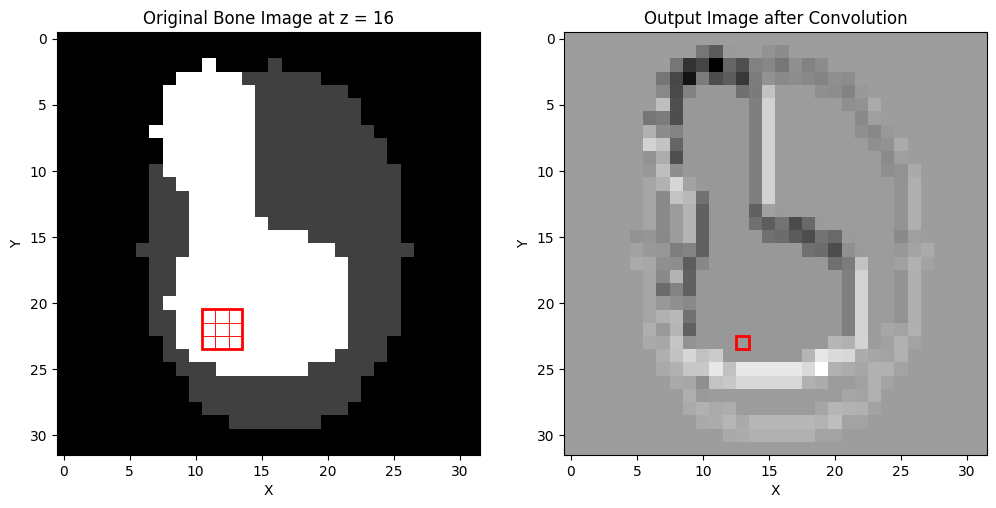
\includegraphics[width=0.7\linewidth]{files/53dfddea48d84244f37a3a2bae253fa3.png}
\caption[]{\textit{left :} original phantom with a 2D 3x3 randomly initialised kernel drawn on top. each individual square represents a pixel, with the outer square representing the kernel. \textit{right :} phantom after 2D convolution layer has been applied.}
\label{convex}
\end{figure}

The left part of Figure~\ref{convex} shows a 3x3 convolution kernel (red) placed on a phantom and the right part of the figure shows the imgage of the phantom after the convolution. Even with randomly initialised weights, there is already an edge-detection like pattern.

A CNN typically consists of multiple layers stacked on top of each other, allowing deeper feature extraction. Early layers can detect simple features like edges, while deeper layers can detect more complex structures like shapes and objects.

\subsubsection{Machine learning - U-Net architecture}

Multiple convolution layers can be combined to form an encoder. An encoder reduces the size of the image between each layer using a max pool layer.A max pool layer devides the input into rectangular regions and taks the maximum value from each region, reducing the image size and allowing the network to capture more abstract and higher-level data.

Similarly a decoder can be used to upsample all features back to an output image. A decoder uses deconvolution layers which increases the size of the feature map as more and more features are added back in.

\begin{figure}[!htbp]
\centering
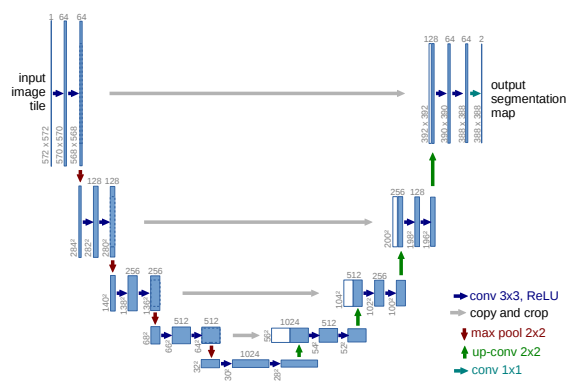
\includegraphics[width=0.75\linewidth]{files/Unet-4562ebe6a22126b0490da719ebbffe48.png}
\caption[]{A Unet architecture for an image with a 32x32 lowest possible resolution. Each blue square represents a multi-channel feature map with the amount of channels denoted on top of the box. Gray arrows represent cross over layers with the white boxes representing copied layers from the encoder \textit{Figure reproduced from} \parencite{oktay2018attention}}
\label{unet}
\end{figure}

Figure~\ref{unet} shows a Unet architecture, which combines an encoder and a decoder with an equal amount of layers. Between each layer of the encoder and decoder part of the network, there is a skip-connection layer as well which copies the feature map from the encoder layer to the decoder layer. This allows the decoder to use features which might have been lost while encoding the image.

\subsubsection{Machine learning - Attention gate}

For feature extraction from images where both local and non-local features are of importance, convolution layers can be combined with attention mechanisms. An attention mechanism is a technique used in machine learning used to allow machine learning models to attend to the most relevant parts of the input data \parencite{vaswani2017attention}.

An attention mechanism takes the input vector $x_{i}^{l}$ and multiplies it by an attention score $\alpha_{i}^{l}$. To get there an intermediate attention score $q_{\text{att}}^{l}$ (the attention score $q_{\text{att}}$ for layer l) can be defined as
\begin{equation}
q_{\text{att}}^{l} = \psi^{T} \, \sigma \left( W_{x}^{T} x_{i}^{l} + W_{g}^{T} g_{i} + b_{g} \right) + b_{\psi}
\end{equation}
where $g_{i}$ the gating feature vector, $W_{x}^{T}$ and $W_{g}^{T}$ weight matrices similar to those used in equation (\ref{denseLayer}), $\psi^{T}$ another linear transformation and $\sigma$ an activation function. The final attention coefficient $\alpha_{i}^{l}$, the final attention mask that says which parts of the feature map should be passed forward, is then calculated as

\begin{equation}
\alpha_{i}^{l} = \sigma_{2} \left( q_{\text{att}}^{l}(x_{i}^{l}, g_{i}; \Theta_{\text{att}}) \right)
\end{equation}
with {\textbackslash}Theta\_\{{\textbackslash}text\{att\}\} representing the learned parameters of the attention block: all weights and biases. The final output of the attention gate it

\begin{equation}
\tilde{x}_i^l = \alpha_i^l \cdot x_i^l
\end{equation}

where regions get $\alpha = 1$ where less important regions get $\alpha \approx 0$

\subsubsection{Machine learning - Attention U-Net}

Attention mechanisms can be added to the skip-connections of the U-Net model in Figure~\ref{unet}, which allows the network to focus on non-local features during the reconstruction of the image. The combination of attention mechanism and convolutional layers can be used to recognise certain features like edges and to easily recognise the link between edges in different parts of the image \parencite{oktay2018attentionunet}.

\begin{figure}[!htbp]
\centering
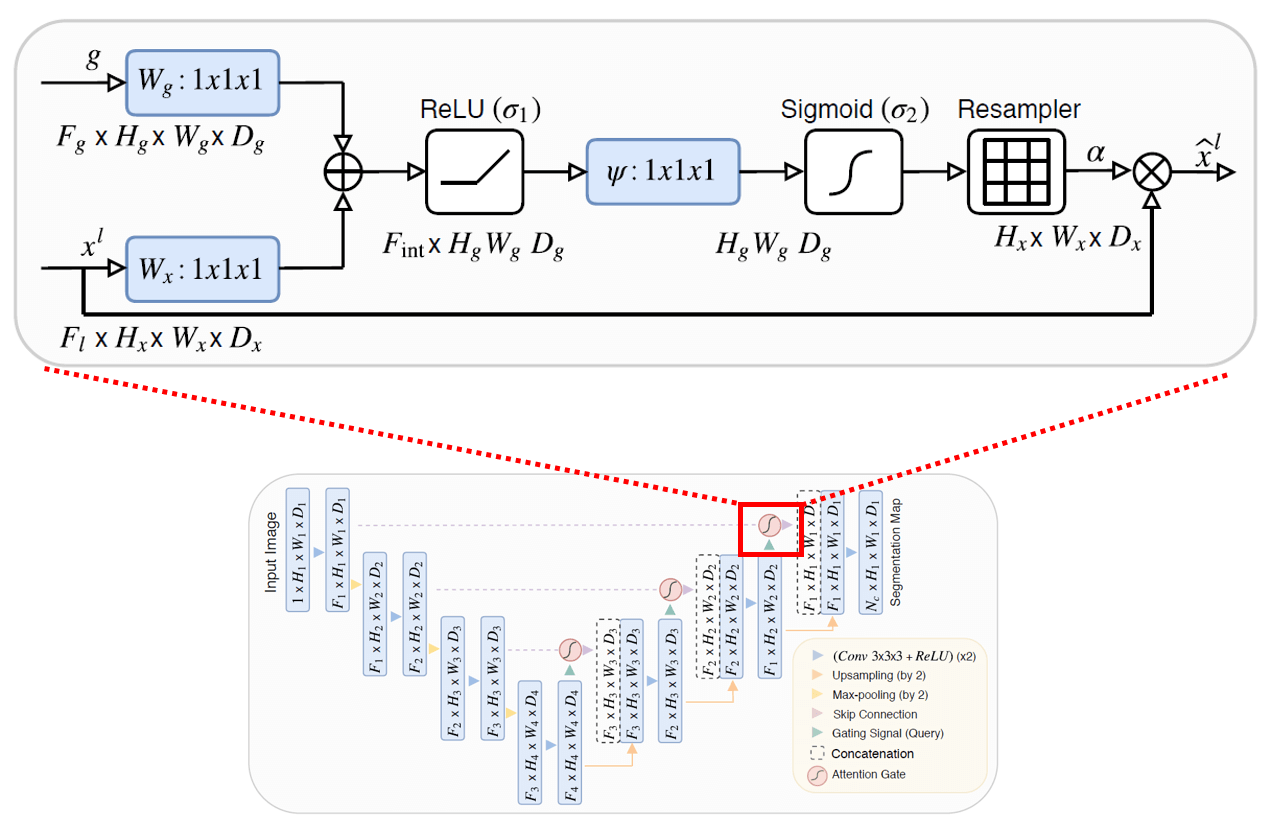
\includegraphics[width=0.7\linewidth]{files/AttU-Net-e5674d1249ce69c5432a1014cf57214e.png}
\caption[]{Schematic overview of a U-Net model with attention gates added to the skip-connections. The inset (top) shows a zoomed-in view of an attention gate, the gating signal $g$ is taken from the previous decoding layer and the input $x^l$ is the skip-connection layer. \textit{Figure reproduced from} \parencite{oktay2018attentionunet}}
\label{attunet}
\end{figure}

The gate vector $g$, also called the gating signal, for each skip-connection layer connects the output of the previous decoder layer to the skip-connection input vector. This is illustrated in Figure~\ref{attunet}.

\begin{figure}[!htbp]
\centering
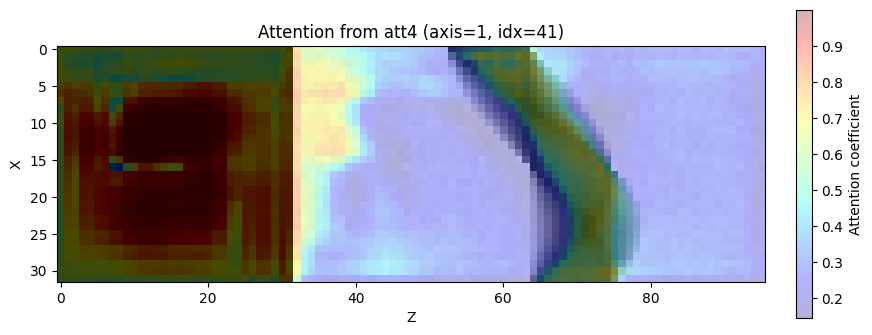
\includegraphics[width=0.7\linewidth]{files/61e001e87d8f0264596b2282806f90e4.png}
\caption[]{An attention map showing how an attention mechanism can be used to have the model focus more on important features, which in this case is the sinogram.}
\label{attention_network}
\end{figure}

Figure~\ref{attention_network} shows an attention map from a trained AttU-Net model. For this specific application it is as expected the attention gate focuses on the lower-intensity parts of the sinogram as these areas provide the most information about the imaged object.

\subsection{Method}

\subsubsection{Generating phantoms}

The phantoms, as illustrated in Figure~\ref{phantomSinogram}, are randomly generated according to a set of rules:

\begin{itemize}
\item each phantom is 32x32x32 pixels and consists of 2 channels, one for bone and one for water.
\item each phantom has a main, elliptical body centered in the image consisting of a low mass density of both water and bone
\item The center of the body can be randomly offset by -3 to +3 pixels in both the x and y directions (uniform distribution).
\item The size of the main body varies, with the distance between the points on the axis varying between 1 and 3 pixels uniformly distributed.
\item each phantom has 2 internal features, represented as smaller elliptical regions within the main body.
\item the bone and/or water density cannot be lower in a feature than the main body
\end{itemize}

Each feature represents a distinct elliptical region. Because photon counting detectors (PCDs) allow differentiating tissue types, we assign one feature a higher bone density and the other a higher water density. This design ensures that the network is trained on a task relevant to the clinical use of PCDs.

Due to constraints within the iterative reconstruction algorithm, the bone and water densities of the features are restricted to be higher than those of the main body.

\subsubsection{acquiring data}

A machine learning model will be trained to use information from sinogram space to adjust images in image space. The network will be trained to perform this conversion in iterative steps similar to an iterative reconstruction method \parencite{mechlem2018joint}.
First, simulations will be run on the randomly generated phantoms. For each phantom, detector measurements will be simulated for x-rays at multiple energy levels: ... kV, ... kV and ... kV. These measurements are done with 32 projections per phantom. An example phantom can be seen in Figure~\ref{phantomSinogram}, with a corresponding sinogram. (which energies?).

Next, each set of detector measurements will be reconstructed using an iterative algorithm with 40 iterations. These iterations will be converted to input-output pairs for training the model. Using a stride, the input is defined as the image from the nth iteration, and the corresponding output image is taken from the (n+stride)th iteration.

Using a stride between input and output images allows the model to learn from a wider variety of scenarios within the same training time. In this work, a stride of 4 is used. This work made use of ... phantoms, which generated ... input-output pairs using a stride of 4 .

\subsubsection{Attention based UNet}

To enable the network to learn the correspondence between features in the image space and the projection (sinogram) space, we employ a UNet architecture with attention mechanisms integrated into the skip connections. The attention gates help the model to focus on which parts of the sinogram contribute to specific image regions.

This work uses a U-Net architecture with attention mechanisms added to the skip-connections as illustraded in Figure~\ref{attunet}. The architecture consists of five convolutional encoder blocks, a bottleneck block, and four decoder blocks. The number of channels increases through the encoder (64 \rightarrow 128 \rightarrow 256 \rightarrow 512 \rightarrow 1024), and then decreases symmetrically through the decoder. The output layer applies a sigmoid activation to produce voxel-wise probabilities.

The model is trained on an NVDIA Tesla A100, with 4 hours allocated per run. The model uses MSELoss as a loss function and Adam optimisation, which is a stochastic gradient descent method. [source] The learning rate is set to 0.001, which is commonly used with Adam optimisation.

\subsubsection{shaping the data}

A U-Net takes an image as an input and provides an image as an output. As 2 different images are used (image and projection) these images have to be appended into a single matrix. Aditionally, due to the pooling layer all dimensions must be powers of 16 as to not get an uneven amount of devisions. The projection matrix is 32 x 44 x 64 pixels, which we can pad with zeros to 32x48x64. The image will is 32 x 32 x 32 pixels which we can pad to 32 x 48 x 32 to fit the dimensions of the projections. The final input set to the network will be 10 x 32 x 48 x 96 as we have 10 channels as well.

\begin{figure}[!htbp]
\centering
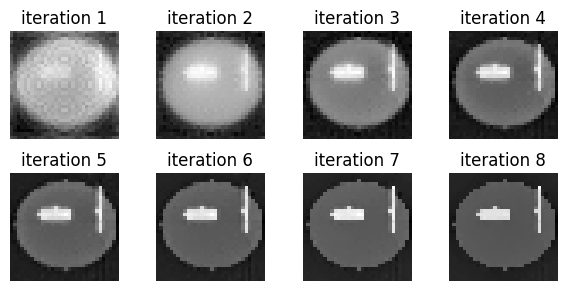
\includegraphics[width=0.7\linewidth]{files/47a8d42f599e527b323d72763db15f1e.png}
\caption[]{Set of iterations from the reconstruction of the bone image of a phantom using stride = 4. The phantom has 2 features with a higher concentration of bone.}
\label{iteration}
\end{figure}

// matching shapes

The projection matrix will have the dimensions of the number of projections x y pixels detector x z pixels detector. The images during reconstruction refer to the intermediate images between each iteration of the iterative algorithm. As both parts of the data have a 3D format, the images will be padded with zeros to match the y-dimension of the projection matrix. The image and the projection are appended in the z-direction.

\subsection{results}

\subsubsection{speedup reconstruction}

During evaluation the model has been run on 20 validation sets constructed with the same rules as the training data. By calculating the root mean square (RMS) error at each iteration for both the iterative algorithm and the model with the ground truth (GT) image, we can compare reconstruction error as a function of time.

\begin{figure}[!htbp]
\centering
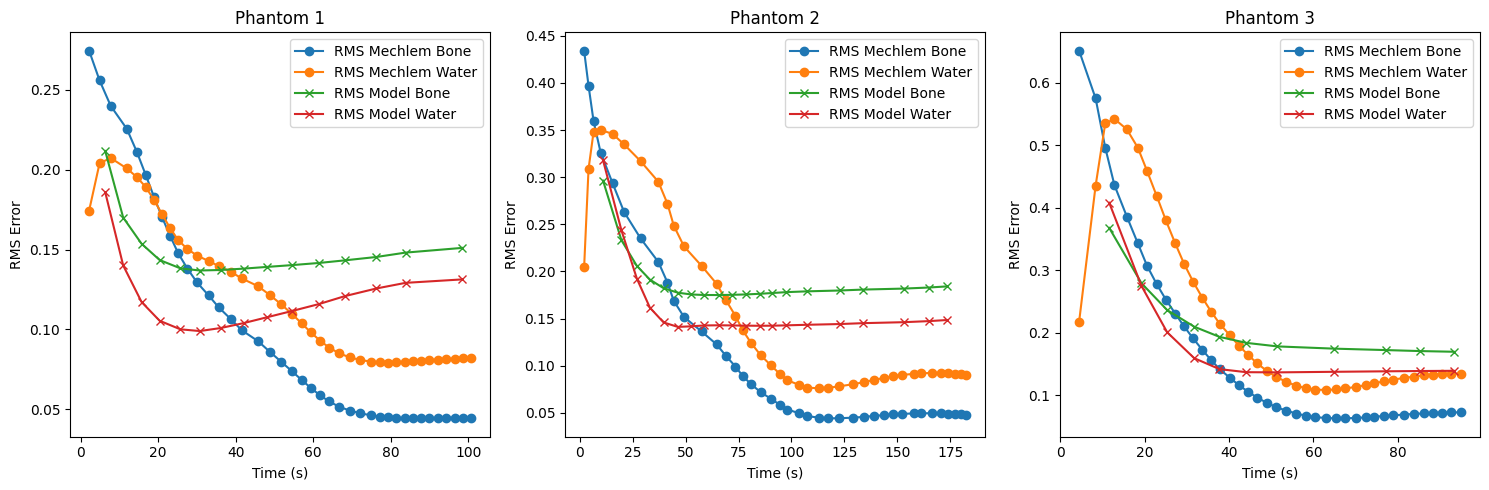
\includegraphics[width=0.7\linewidth]{files/ece13eed65e4da5e0fcfb17c55d81ea7.png}
\caption[]{RMS error over time for three phantoms reconstructed using both the iterative method (orange: water; blue: bone) and the proposed model (red: water; green: bone).}
\label{rmsTime}
\end{figure}

Figure~\ref{rmsTime} shows the RMS error over time for bone and water images reconstructed by both methods for 3 phantoms. The model has been cut off after the iterative algoritm stopped running for phantom 1 and 3. In all three cases, the model achieves a lower initial error but converges to a bigger error compared to the iterative algorithm. For both algorithms the RMS error of the water images converges to a higher value than the RMS of the bone images.

\begin{figure}[!htbp]
\centering
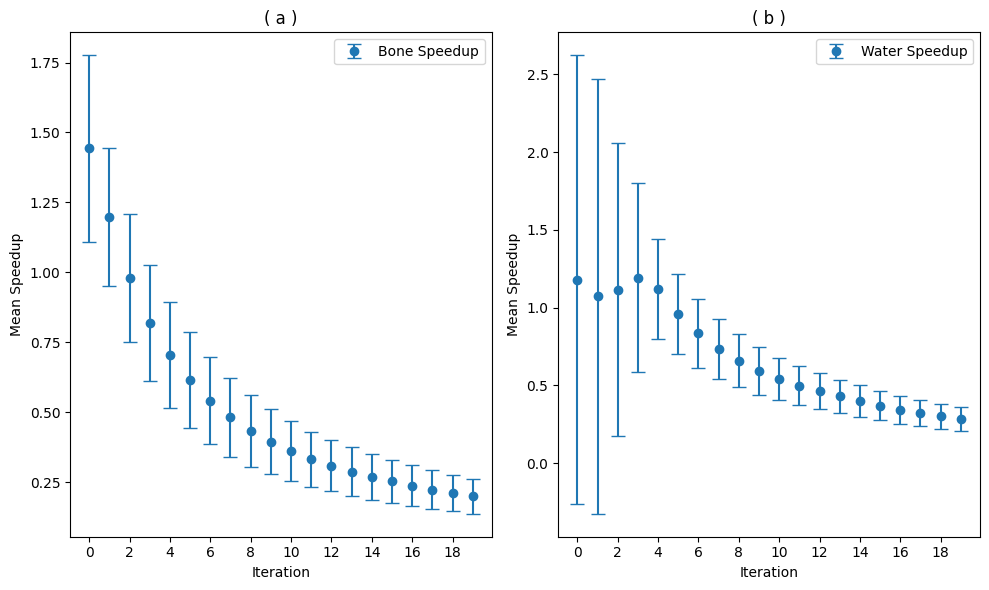
\includegraphics[width=0.7\linewidth]{files/2736d68d407f8ad6de225a7e5df53bf4.png}
\caption[]{The RMS-error plotted against time for 3 phantoms reconstructed using both the iterative method as well as the model. For both methods, the RMS is calculated for the bone and water image.}
\label{speedup_interpolated}
\end{figure}

Looking at a dataset of 20 phantoms, the average time taken for the first iteration of the model is 9.3 seconds with a standard deviation of 1.5 seconds. The average speedup for bone for this step (how long it takes the iterative algorithm to get to the same RMS error) is 1.44 times, or 44\% while the average speedup for water is 1.17 times, or 17\%. As the average time per iteration has a standard deviation of 1.5 seconds, the average speedup can be plotted against iteration of the proposed model as illustrated in Notebook-code.

\subsubsection{Visualise reconstruction}

To further understand the results we can look at a specific reconstruction.

\begin{figure}[!htbp]
\centering
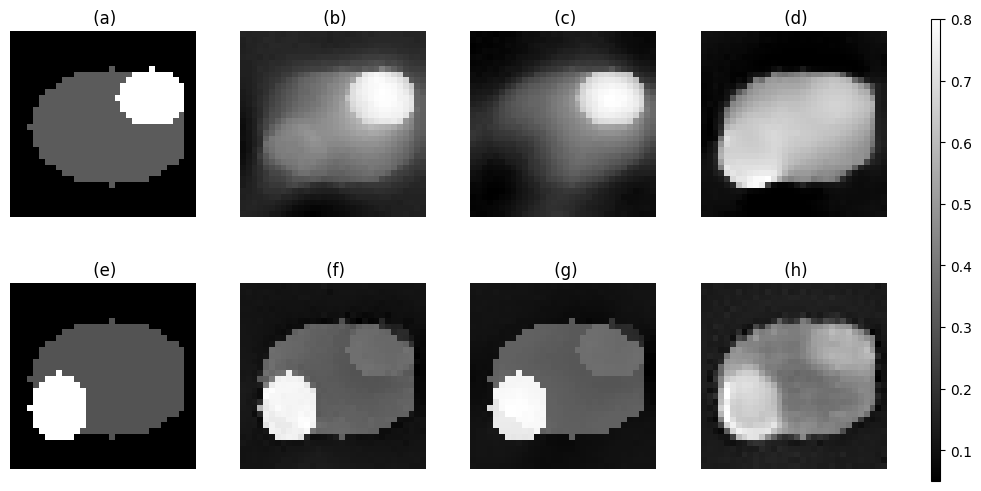
\includegraphics[width=0.7\linewidth]{files/bdda59cec4f2e4c72b6b8b7af0f49ee7.png}
\caption[]{(a) GT water image (b) smallest RMS water image iterative algorithm (c) water image from last iteration iterative algorithm (d) water image reconstructed by the model after 3 iterations (e) GT bone image (f) smallest RMS bone image iterative algorithm (g) bone image from last iteration iterative algorithm (h) bone image recontructed by the model after 3 iterations.}
\label{reconPhantom}
\end{figure}

Figure~\ref{reconPhantom} shows the GT for water and bone and the corresponding reconstructions. Aside from the final reconstruction it is important to look at the reconstruction with the lowest error of the iterative approach. The ground truth (GT) consists of a bone feature in the lower left part of the image and a water feature in the top right part of the image. Starting with water, the most accurate reconstruction shows signs of both features. The last iteration however shows a larger bone density for the water feature but the algortithm seems to have overcompensated by fully removing the water density for the feature in the bottom left.

\subsubsection{wrong reconstructions}

potentially display another set of reconstructions which are not good to highlight the inconsistency in the training data

\subsection{Discussion}

\subsubsection{non-machine learning speedup}

\begin{itemize}
\item pytorch is highly optimized, mechlem is not
\item
\end{itemize}

\subsubsection{pixel size and number of projections necessary}

There will not be a linear relationship between the amount of projections necessary and the amount of pixels in the image. will this have an impact?

\subsubsection{Model is only as good as your data}

Looking at the accuracy of the model

\subsubsection{Adding cross attention between spaces}

\begin{itemize}
\item adding cross attention can more accuratly predict which part of the sinogram attend to which parts of the image. Then convolution can still be used to reconstruct the image.
\end{itemize}

\section{Conclusion}

\printbibliography

% DON'T EDIT. If "endfloat" option is enabled all floats appear before appendices
\if@endfloat\clearpage\processdelayedfloats\clearpage\fi


%%%%%%%%%%%%%%%%%%%%%%%%%%%%%%%%%%%%%%%%%%%%%%%%%%%%%%%%%%%%
%%% SUPPLEMENTARY MATERIAL / APPENDICES
%%%%%%%%%%%%%%%%%%%%%%%%%%%%%%%%%%%%%%%%%%%%%%%%%%%%%%%%%%%%
%% Sadly, we can't use floats in the appendix boxes. So they don't "float", but use \captionof{figure}{...} and \captionof{table}{...} to get them properly caption.

%%%%%%%%%%%%%%%%%%%%%%%%%%%%%%%%%%%%%%%%%%%%%%%%%%%%%%%%%%%%
%%% ARTICLE END
%%%%%%%%%%%%%%%%%%%%%%%%%%%%%%%%%%%%%%%%%%%%%%%%%%%%%%%%%%%%

\end{document}
